\documentclass[preview,convert={convertexe={magick},outext=.ps}]{standalone}
\usepackage[dvipdfm]{geometry}
\usepackage{xcolor}
\usepackage[caption=false,font=footnotesize]{subfig}
\usepackage{tikz}
\usetikzlibrary{shapes.geometric, shapes.multipart, arrows, calc, through,intersections}


\begin{document}
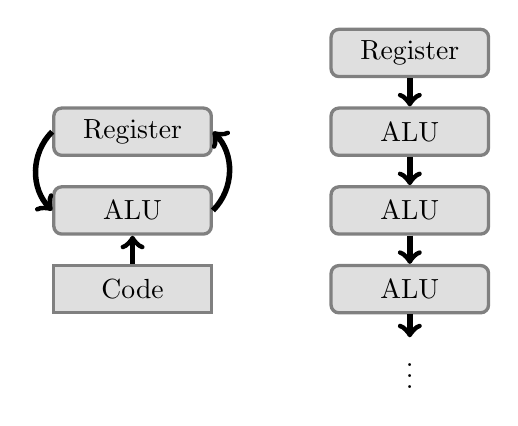
\begin{tikzpicture}[
node distance=10mm,
elem/.style={
    rectangle,minimum width=2cm,minimum height=6mm,rounded corners=1mm,very thick,draw=black!50,fill=lightgray!50
},
code/.style={
    rectangle,minimum width=2cm,minimum height=6mm,very thick,draw=black!50,fill=lightgray!50
}
]
    \node(N1)[elem]{Register};
    \node(N2)[below of=N1,elem]{ALU};
    \node(N3)[below of=N2,code]{Code};
    \draw[->,bend right=45,line width=2pt] (N1.west) to (N2.west);
    \draw[<-,bend left=45,line width=2pt] (N1.east) to (N2.east);
    \draw[->,line width=2pt] (N3.north) to (N2.south);
    
    \node(M1)[elem] at ($(N1.east)+(2.5,1)$){Register};
    \node(M2)[elem,below of=M1]{ALU};
    \node(M3)[elem,below of=M2]{ALU};
    \node(M4)[elem,below of=M3]{ALU};
    \node(M5)[rectangle,below of=M4]{\vdots};
    \draw[->,line width=2pt] (M1.south) to (M2.north);
    \draw[->,line width=2pt] (M2.south) to (M3.north);
    \draw[->,line width=2pt] (M3.south) to (M4.north);
    \draw[->,line width=2pt] (M4.south) to (M5.north);
\end{tikzpicture}
\end{document}
